\documentclass{article}

\usepackage{polski}
\usepackage{amsmath}
\usepackage{graphicx}
\usepackage{array}
\setlength{\extrarowheight}{.5ex}
\usepackage{float}
\usepackage{xcolor}

\newsavebox\MBox
\newcommand\Cline[2][red]{{\sbox\MBox{$#2$}%
  \rlap{\usebox\MBox}\color{#1}\rule[-1.2\dp\MBox]{\wd\MBox}{0.5pt}}}

\title{Sprawozdanie 3: Liczniki i automaty}

\author{\textbf{Jakub Szymczak, Damian Tworek,}\\ \textbf{Maksymilian Sulima, Łukasz Wala} \\
    \textit{AGH, Wydział Informatyki, Elektroniki i Telekomunikacji} \\
    \textit{Technika Cyfrowa 2021/2022}}
\date{Kraków, \today}

\begin{document}
\maketitle

\section{Ćwiczenie \textit{3a}}
Ideą ćwiczenia jest zaprojektowanie, zrealizowanie i przetestowanie dwójki liczącej w oparciu o przerzutnik JK. 

\begin{figure}[H]
    \centering
    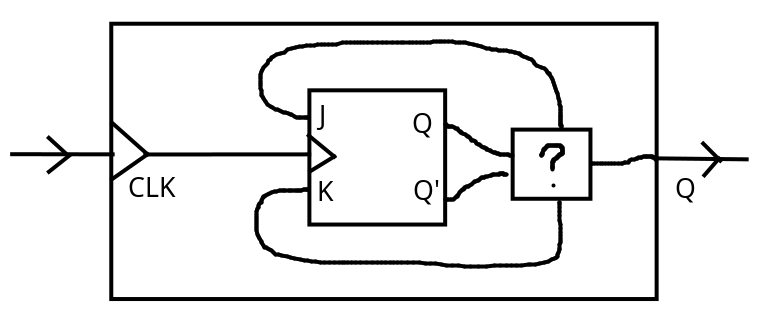
\includegraphics[width=0.5\textwidth]{3a_idea_1.jpg}
    \caption{Dwójka licząca}
\end{figure}

Układ ma wejście zegara \textbf{CLK} oraz wyjście \textbf{Q}. W kolejnych taktach zegara stan na wyjściu \textbf{Q} zmienia się na przeciwny.

Następnie w oparciu o jeden z wariantów zaprojektowanej dwójki liczącej, zaprojektowany i przetestowany zostanie asynchroniczny licznik
modulo 8.

\begin{figure}[H]
    \centering
    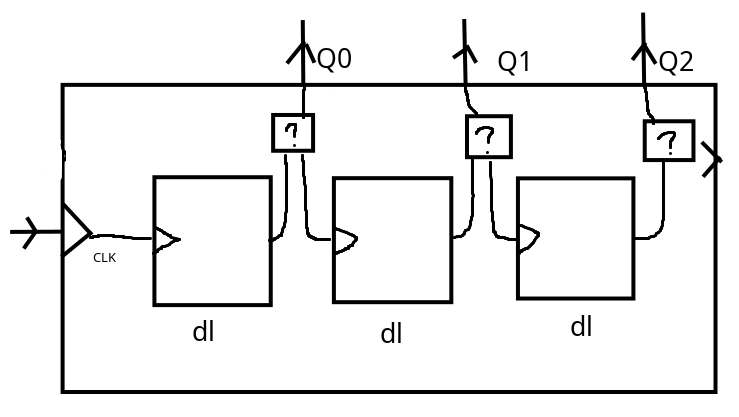
\includegraphics[width=0.4\textwidth]{3a_idea_2.jpg}
    \caption{Asynchroniczny licznik modulo 8}
\end{figure}

Wejście zegara oznaczono jako \textbf{CLK}, natomiast wyjścia to (w kolejności od najmniej istotnego bitu) 
\textbf{Q0}, \textbf{Q1}, \textbf{Q2}.

\subsection{Rozwiązanie teoretyczne}

Tabela prawdy dla dwójki liczącej wygląda następująco:

\begin{figure}[H]
    \centering
    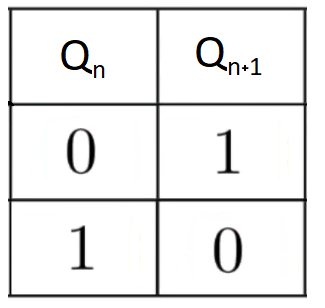
\includegraphics[width=0.2\textwidth]{3a_tabela_prawdy.png}
    \caption{Tabela prawdy dla dwójki liczącej}
\end{figure}

Do zbudowania jej będzie potrzebny jeden przerzutnik JK:

\begin{figure}[H]
    \centering
    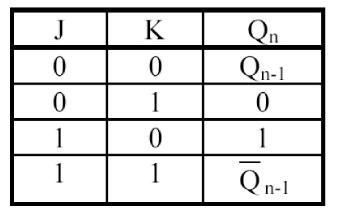
\includegraphics[width=0.4\textwidth]{3a_prawda_o_JK.png}
    \caption{Tabela prawdy dla przerzutnika JK}
\end{figure}

Na podstawie tych dwóch tabel można wywnioskować, które stany przerzutnika JK będzie można wykorzystać (z możliwych kombinacji wybrane
zostały dwie):

\begin{figure}[H]
    \centering
    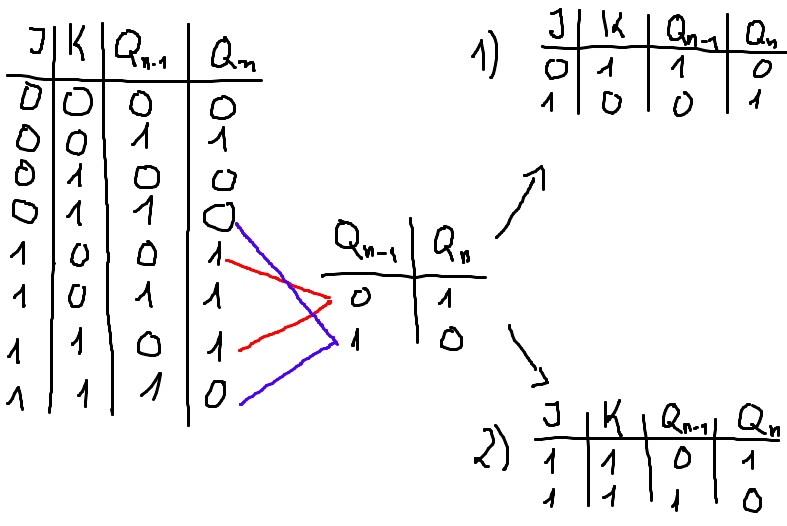
\includegraphics[width=0.8\textwidth]{3a_teor1.jpg}
    \caption{Rozwiązanie teoretyczne}
\end{figure}

\pagebreak
Tabele Karnough dla pierwszego przypadku:

\begin{figure}[H]
    \centering
    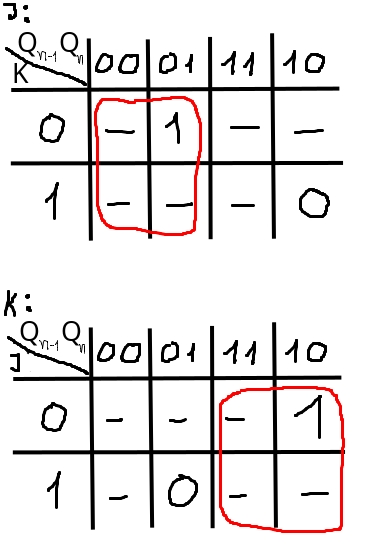
\includegraphics[width=0.4\textwidth]{3a_kar_1.jpg}
    \caption{Tabela Karnough dla przypadku 1}
\end{figure}

Można zauważyć, że $Q_{n-1}$ jest zawsze równe $\overline{Q}$, więc można skorzystać z wyjścia zanegowanego wyjścia \textbf{Q} w przerzutniku\
JK.

$$J=Q_{n-1}=\overline{Q}$$
$$K=Q_n$$

\begin{figure}[H]
    \centering
    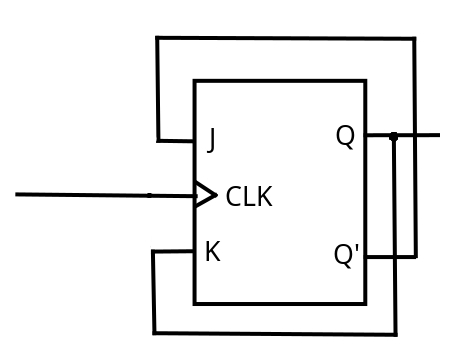
\includegraphics[width=0.6\textwidth]{3a_model_1.jpg}
    \caption{Schemat dla tabeli 1}
\end{figure}

\pagebreak
Tabela Karnough dla drugiego przypadku:

\begin{figure}[H]
    \centering
    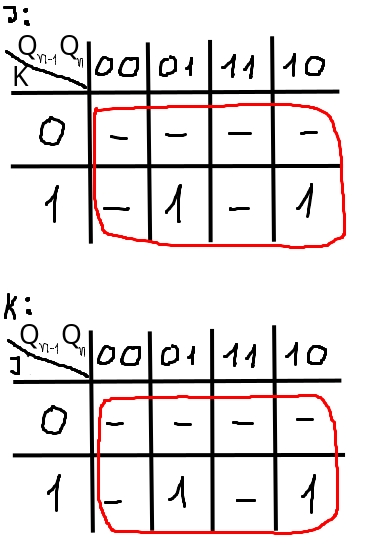
\includegraphics[width=0.4\textwidth]{3a_kar_2.jpg}
    \caption{Tabela Karnough dla przypadku 2}
\end{figure}

$$J=1$$
$$K=1$$

\begin{figure}[H]
    \centering
    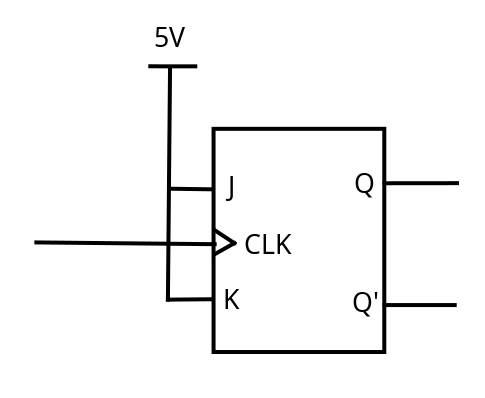
\includegraphics[width=0.7\textwidth]{3a_model_2.jpg}
    \caption{Schemat dla tabeli 2}
\end{figure}

\subsection{Implementacja w programie Multisim}
Poniżej znajduje się implementacja obu wariantów układu:

\begin{figure}[H]
    \centering
    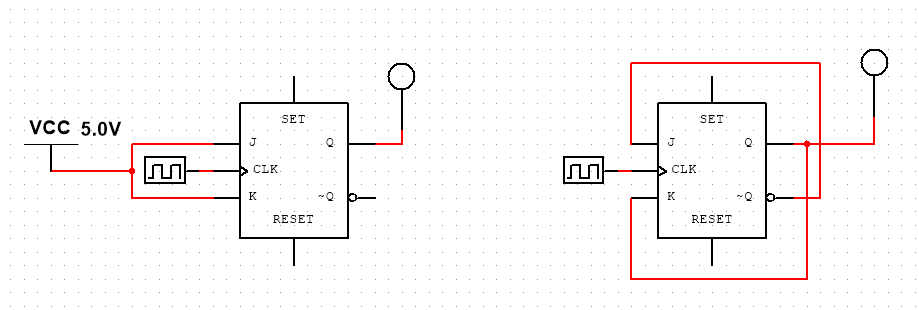
\includegraphics[width=\textwidth]{3a_dwojka.png}
    \caption{Implementacja dwójki liczącej}
\end{figure}

Układ testujący dla dwójki liczącej (używający wariantu po lewej stronie):

\begin{figure}[H]
    \centering
    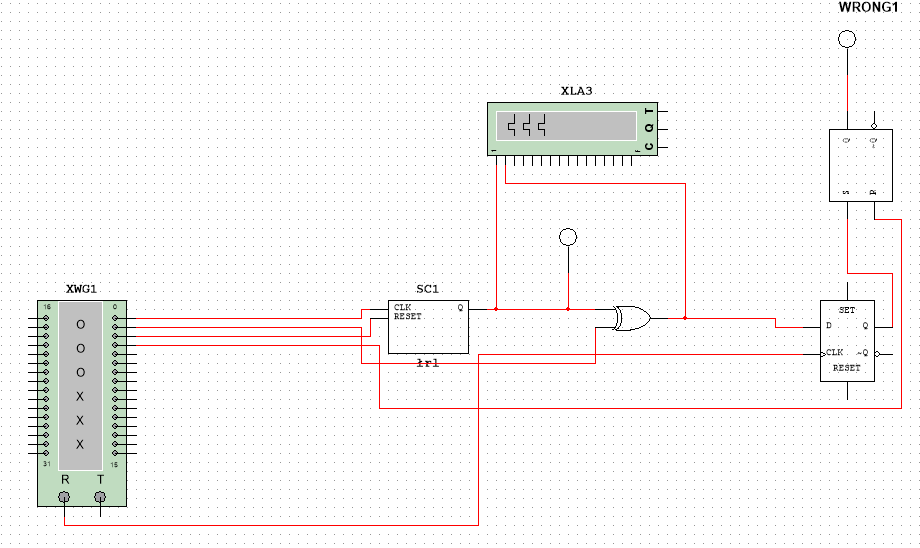
\includegraphics[width=\textwidth]{3a_dwojka_test.png}
    \caption{Układ testujący dla dwójki liczącej}
\end{figure}

\begin{figure}[H]
    \centering
    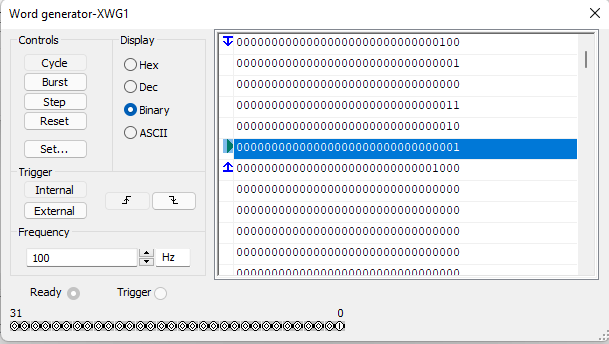
\includegraphics[width=\textwidth]{3a_dwojka_gen.png}
    \caption{Generator słów dla układu testującego}
\end{figure}

\begin{figure}[H]
    \centering
    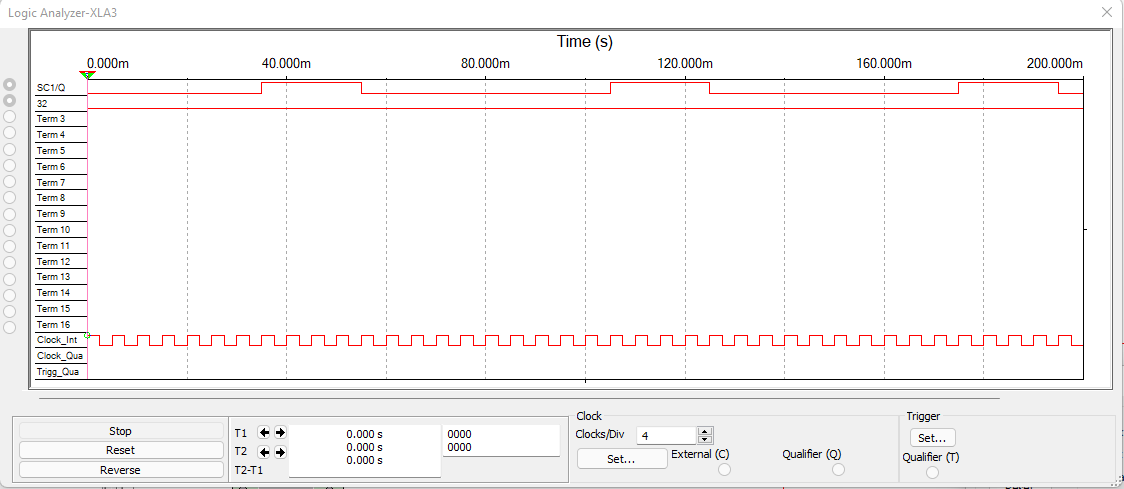
\includegraphics[width=\textwidth]{3a_dwojka_ana.png}
    \caption{Analizator dla układu testującego}
\end{figure}

\begin{figure}[H]
    \centering
    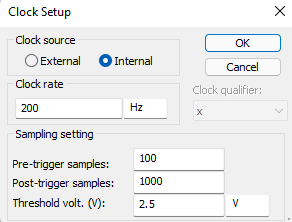
\includegraphics[width=0.3\textwidth]{3a_dwojka_anasetup.png}
    \caption{Ustawienia analizatora}
\end{figure}

\subsection{Asynchroniczny licznik modulo 8}
Asynchroniczny licznik modulo 8 (odliczający do góry 0,1,2,...,7) można stworzyć używając trzech dwójek liczących, łącząc ich zanegowane wyjścia z wejściami
zegara kolejnych (tylko, gdy użyty przerzutnik JK reaguje na wzrastający sygnał zegara):

\begin{figure}[H]
    \centering
    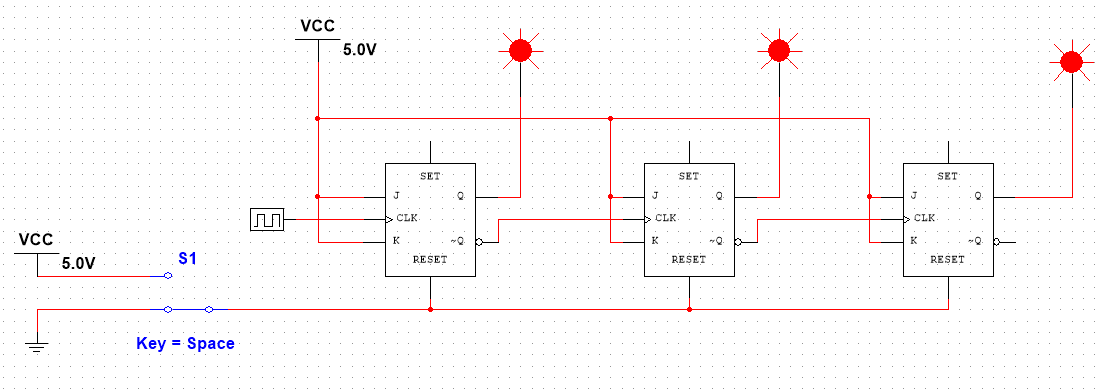
\includegraphics[width=\textwidth]{3a_modulo8.png}
    \caption{Implementacja asynchronicznego licznika modulo 8}
\end{figure}

\pagebreak
Poniżej układ testujący:

\begin{figure}[H]
    \centering
    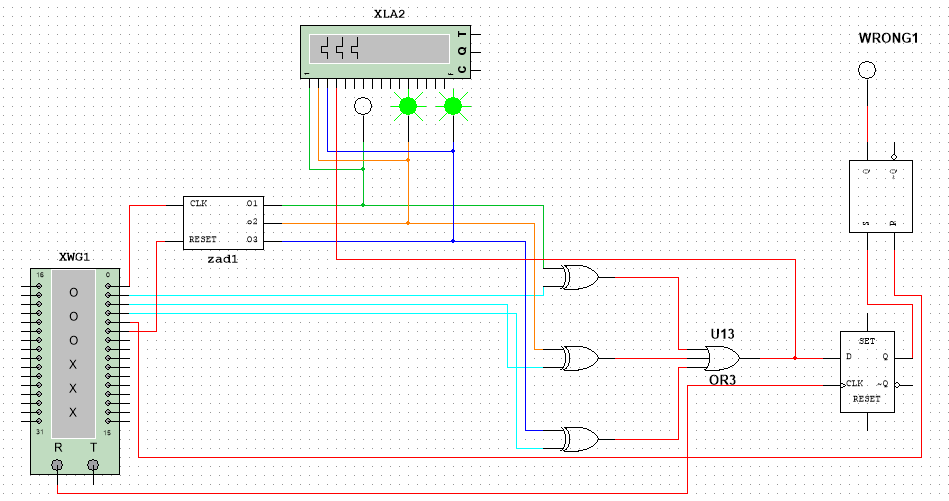
\includegraphics[width=\textwidth]{3a_modulo8_test.png}
    \caption{Układ testujący dla asynchronicznego licznika modulo 8}
\end{figure}

\begin{figure}[H]
    \centering
    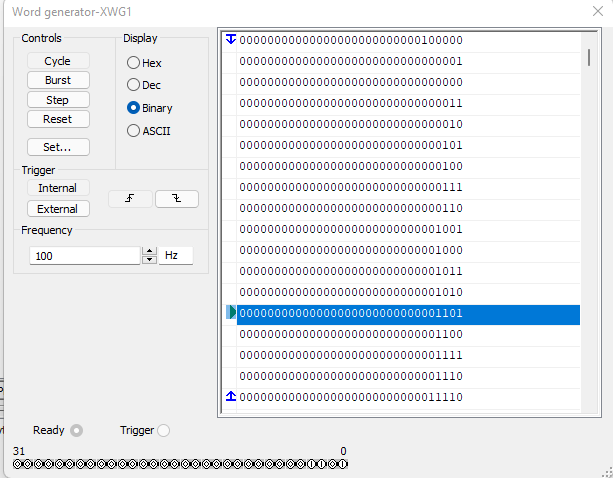
\includegraphics[width=\textwidth]{3a_modulo8_gen.png}
    \caption{Generator słów dla układu testującego}
\end{figure}

\begin{figure}[H]
    \centering
    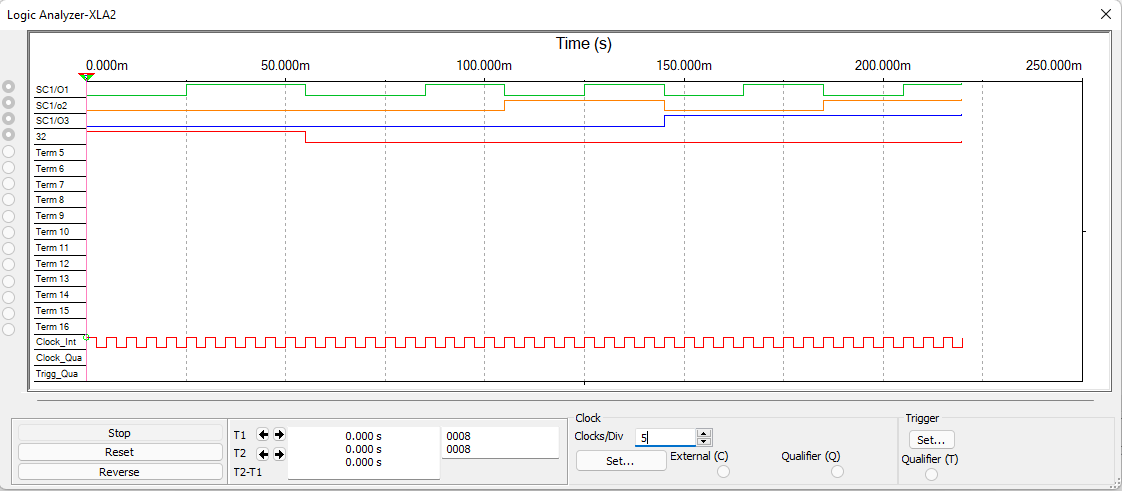
\includegraphics[width=\textwidth]{3a_modulo8_ana.png}
    \caption{Analizator dla układu testującego}
\end{figure}

\begin{figure}[H]
    \centering
    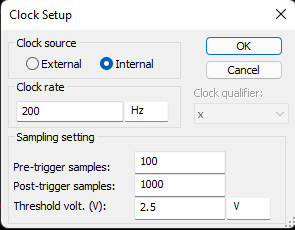
\includegraphics[width=0.5\textwidth]{3a_modulo8_anasetup.png}
    \caption{Ustawienia analizatora}
\end{figure}

\subsection{Wnioski}

\begin{itemize}
    \item
    Liczniki asynchroniczne mają ograniczone zastosowanie, ponieważ, w związku z tym, że przerzutniki sterowane
    są wyjściami przerzutników poprzedzających, 
    stan nie ustala się od razu, więc jeżeli impulsy zegarowe mają dużą częstotliwość i ich okres jest
    porównywalny z czasem propagacji przerzutnika, to sygnały wyjściowe licznika mogą podawać złe wartości.
    Rozwiązaniem tego problemu są liczniki synchroniczne.
    \item
    Dwójki liczącej oraz liczników w ogólności można użyć do zmniejszania częstotliwości zegara (jeżeli dwójka reaguje na
    zmianę z 0 na 1, wówczas częstosliwość na wyjściu zmniejszona jest dwukrotnie).

    \begin{figure}[H]
        \centering
        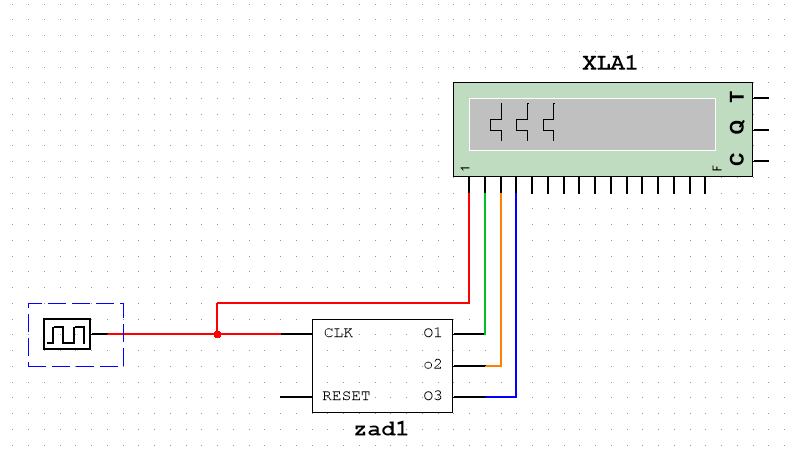
\includegraphics[width=\textwidth]{3a_przyklad_1.png}
        \caption{Układ zmniejszający czętstotliwość}
    \end{figure}

    \begin{figure}[H]
        \centering
        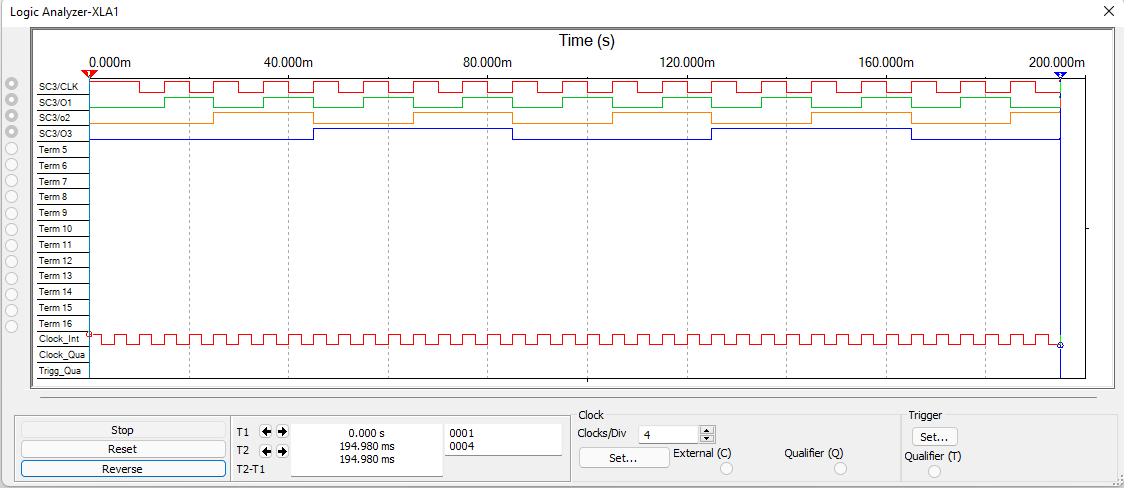
\includegraphics[width=\textwidth]{3a_przyklad_2.png}
        \caption{analizator układu zmniejszającego częstotliwość}
    \end{figure}

    Jak widać, częstotliwość na wyjści najmniej znaczącego bitu jest zmniejszona dwukrotnie, na drugim bicie czterokrotnie itd.

\end{itemize}

\pagebreak
\section{Ćwiczenie \textit{3b}}
Ideą ćwiczenia jest, bazując na dowolnie wybranych przerzutnikach, zaprojektowanie, zbudowanie i przetestowanie synchronicznego
czterobitowego licznika liczącego w kodzie Graya.

\begin{figure}[H]
    \centering
    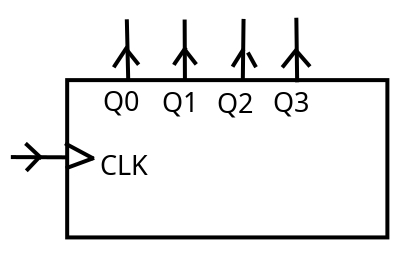
\includegraphics[width=0.4\textwidth]{3b_idea.jpg}
    \caption{Synchroniczny licznik czterobitowy w kodzie Graya}
\end{figure}

\subsection{Rozwiązanie teoretyczne}
Wszystkie układy są synchroniczne i zakładają zmianę stanu przy zmianie sygnału zegarowago.

Licznik powinien liczyć w kodzie Graya, co oznacza, że dwa kolejne stany różnią się dokładnie jednym bitem:

\begin{figure}[H]
    \centering
    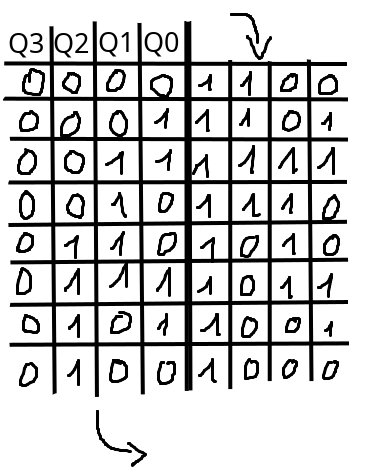
\includegraphics[width=0.4\textwidth]{3b_gray.jpg}
    \caption{Kolejne stany licznika}
\end{figure}

\pagebreak
W implementacji użyte zostaną przerzutniki D:

\begin{figure}[H]
    \centering
    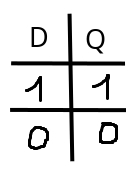
\includegraphics[width=0.2\textwidth]{3b_dtruth.jpg}
    \caption{Tabela przejść dla przrzutnika D}
\end{figure}

Wyjście przerzutnika $D_i$ odpowiada $Q_i$:

\begin{figure}[H]
    \centering
    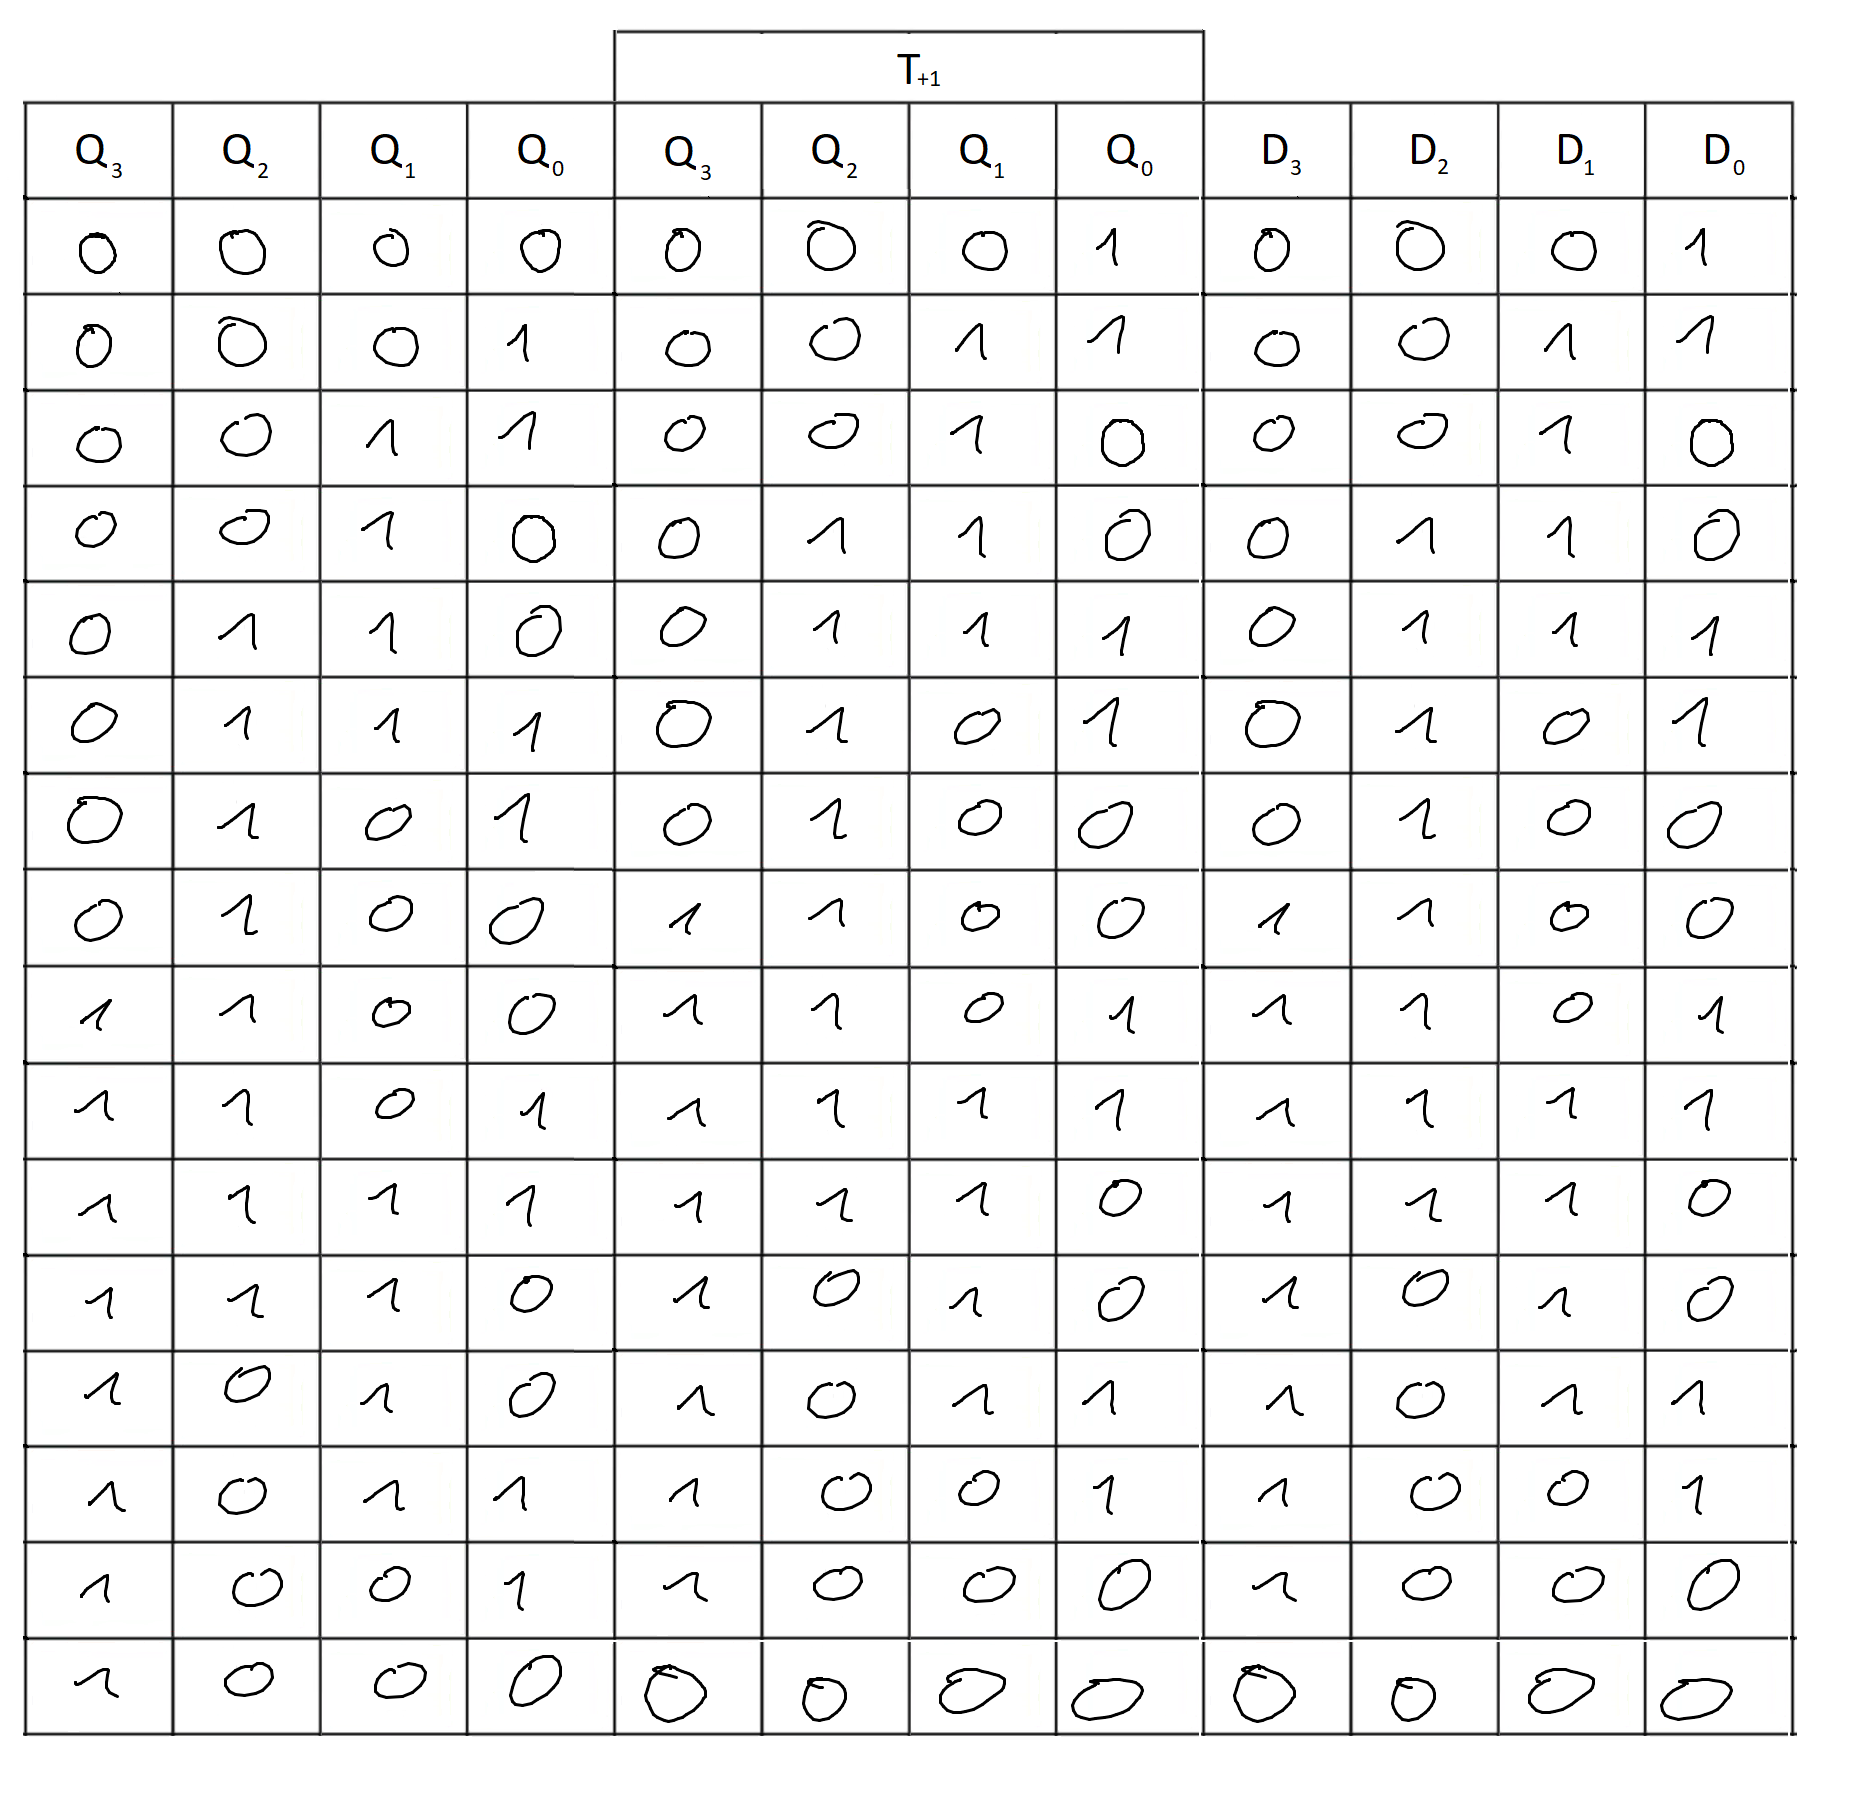
\includegraphics[width=\textwidth]{3b_table.png}
    \caption{Tabela prawdy dla licznika}
\end{figure}

Na podstawie tabeli prawdy licznika można skonstruować tabele Karnough oraz wzory dla $D_0$, $D_1$, $D_2$, $D_3$:

\begin{figure}[H]
    \centering
    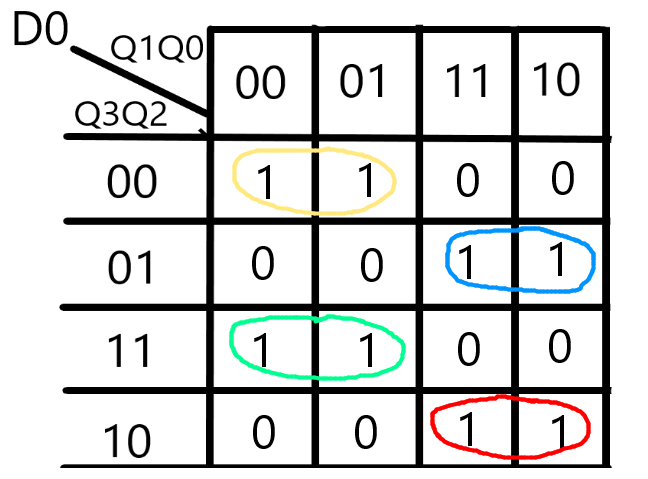
\includegraphics[width=0.5\textwidth]{3b_karn0.png}
    \caption{Tabela Karnough dla $D_0$}
\end{figure}

$$D_0 = \Cline[yellow]{\overline{Q_3}\:\overline{Q_2}\:\overline{Q_1}} + 
\Cline[blue]{\overline{Q_3}Q_2Q_1} + 
\Cline[green]{Q_3Q_2\overline{Q_1}} + 
\Cline[red]{Q_3\overline{Q_2}Q_1}$$

Ten wzór da się uprościć. Korzystając z rozdzielności koniunkcji względem alternatywy

$$D_0 = \overline{Q_3}(\overline{Q_2}\:\overline{Q_1} + Q_2Q_1) + Q_3(Q_2\overline{Q_1} + \overline{Q_2}Q_1)$$

Tutaj natomiast można zauważyć, że zawartość pierwszego nawiasu to wzór na XNOR, a drugiego na XOR, więc

$$D_0 = \overline{Q_3}(\overline{Q_1\oplus Q_2}) + Q_3(Q_1\oplus Q_2)$$

Ponownie, jest to wzór na XNOR $Q_3$ oraz zawartości nawiasu

$$D_0 = \overline{Q_1 \oplus Q_2 \oplus Q_3}$$

\begin{figure}[H]
    \centering
    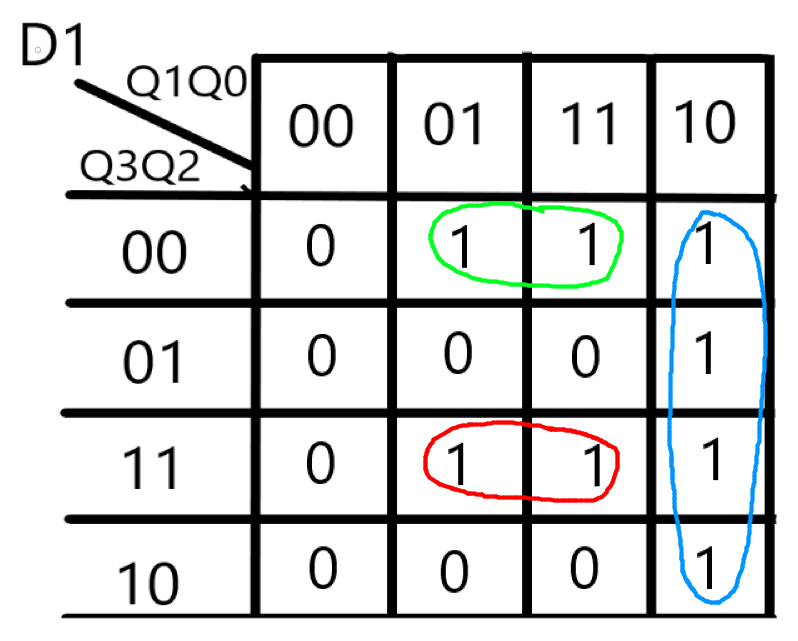
\includegraphics[width=0.6\textwidth]{3b_karn1.png}
    \caption{Tabela Karnough dla $D_1$}
\end{figure}

$$D_1 = \Cline[blue]{Q_1\overline{Q_0}} +
\Cline[green]{\overline{Q_3}\:\overline{Q_2}Q_0} + 
\Cline[red]{Q_3Q_2Q_0}$$

Tutaj można skorzystać z prawa rozdzielności koniunkcji względem alternatywy

$$D_1 = Q_1\overline{Q_0} + Q_0(\overline{Q_2}\:\overline{Q_3} + Q_2Q_3)$$

Zawartość nawiasu to XNOR

$$D_1 = Q_1\overline{Q_0} + Q_0(\overline{Q_2 \oplus Q_3})$$

\pagebreak
\begin{figure}[H]
    \centering
    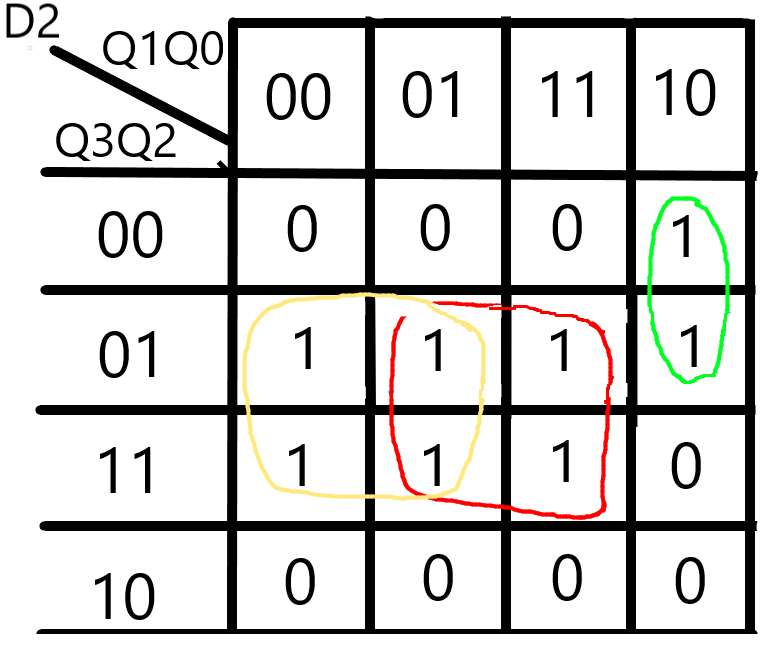
\includegraphics[width=0.6\textwidth]{3b_karn2.png}
    \caption{Tabela Karnough dla $D_2$}
\end{figure}

$$D_2 = \Cline[green]{Q_1\overline{Q_0}\:\overline{Q_3}} +
\Cline[red]{Q_0Q_2} + 
\Cline[yellow]{\overline{Q_1}Q_2}$$

\begin{figure}[H]
    \centering
    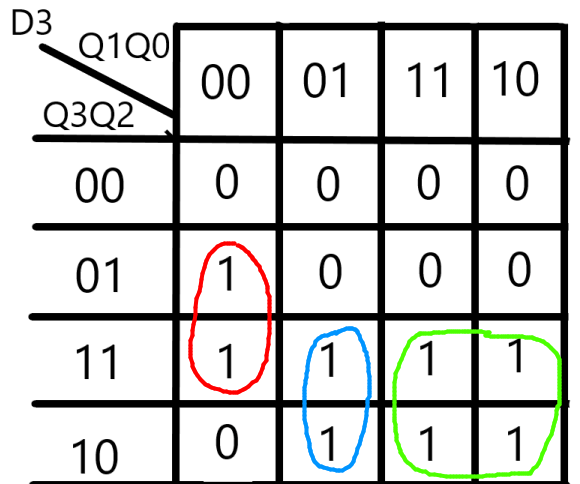
\includegraphics[width=0.6\textwidth]{3b_karn3.png}
    \caption{Tabela Karnough dla $D_3$}
\end{figure}

$$D_3 = \Cline[green]{Q_1Q_3} +
\Cline[blue]{Q_3\overline{Q_1}Q_0} + 
\Cline[red]{Q_2\overline{Q_1}\:\overline{Q_0}}$$

\subsection{Implementacja w programie Multisim}

\begin{figure}[H]
    \centering
    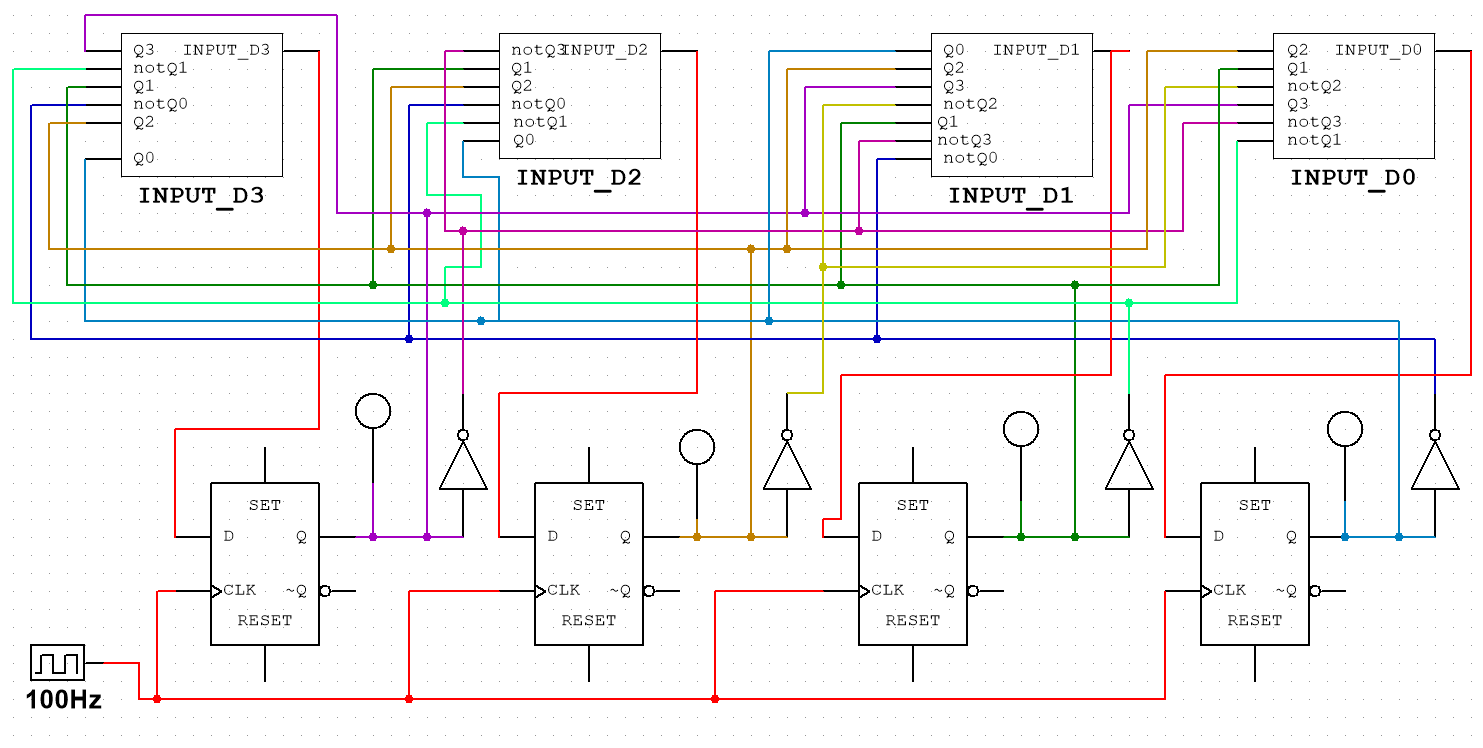
\includegraphics[width=\textwidth]{3b_impl.png}
    \caption{Implementacja licznika}
\end{figure}

$$D_0 = \overline{Q_1 \oplus Q_2 \oplus Q_3}$$

\begin{figure}[H]
    \centering
    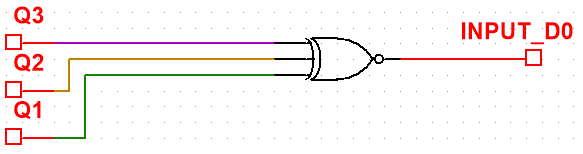
\includegraphics[width=\textwidth]{3b_impl_0.png}
    \caption{Podukład 0}
\end{figure}

\pagebreak
$$D_1 = Q_1\overline{Q_0} + Q_0(\overline{Q_2 \oplus Q_3})$$

\begin{figure}[H]
    \centering
    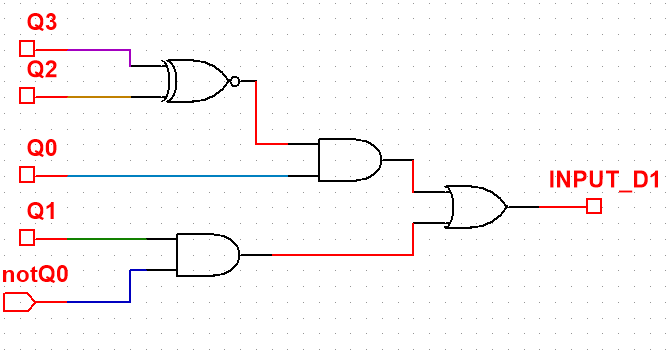
\includegraphics[width=\textwidth]{3b_impl_1.png}
    \caption{Podukład 1}
\end{figure}

$$D_2 = Q_1\overline{Q_0}\:\overline{Q_3} +
Q_0Q_2 + 
\overline{Q_1}Q_2$$

\begin{figure}[H]
    \centering
    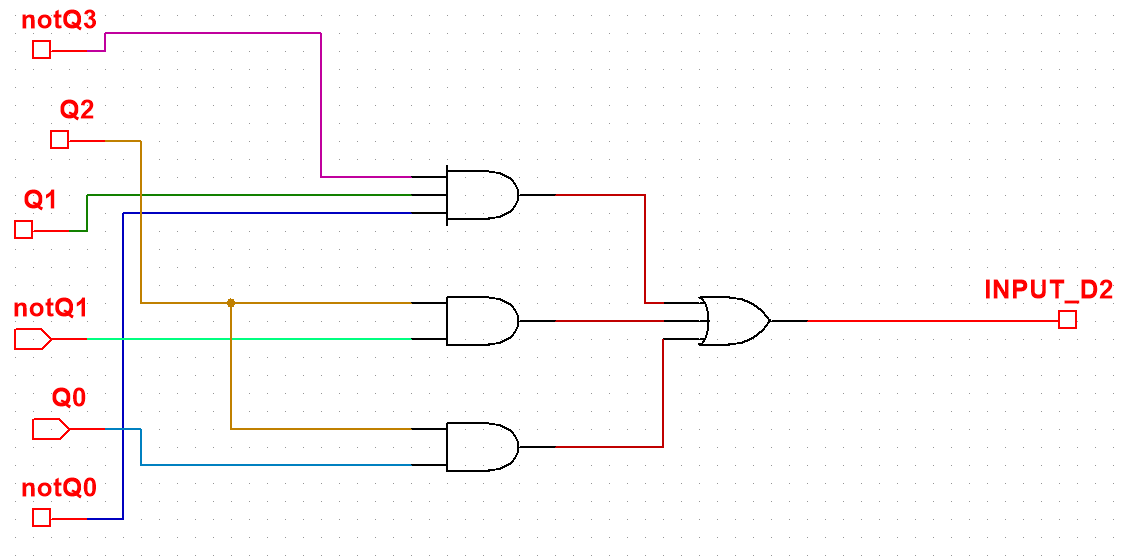
\includegraphics[width=\textwidth]{3b_impl_2.png}
    \caption{Podukład 2}
\end{figure}

\pagebreak
$$D_3 = Q_1Q_3 +
Q_3\overline{Q_1}Q_0 + 
Q_2\overline{Q_1}\:\overline{Q_0}$$

\begin{figure}[H]
    \centering
    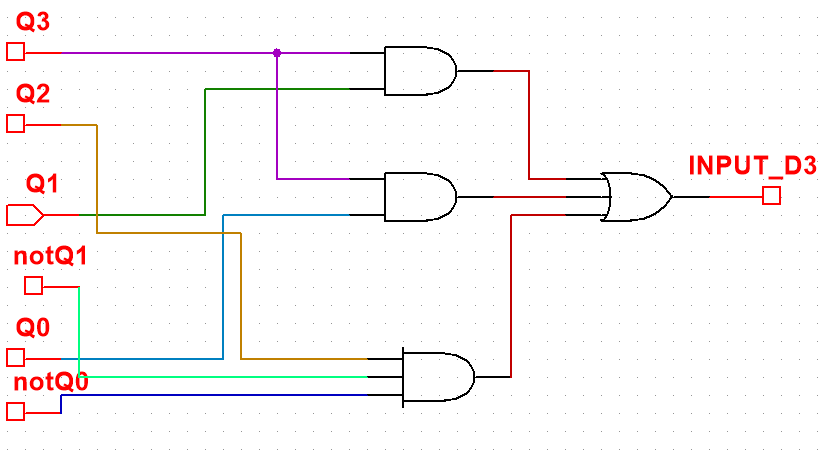
\includegraphics[width=\textwidth]{3b_impl_3.png}
    \caption{Podukład 3}
\end{figure}

Poniżej układ testujący

\begin{figure}[H]
    \centering
    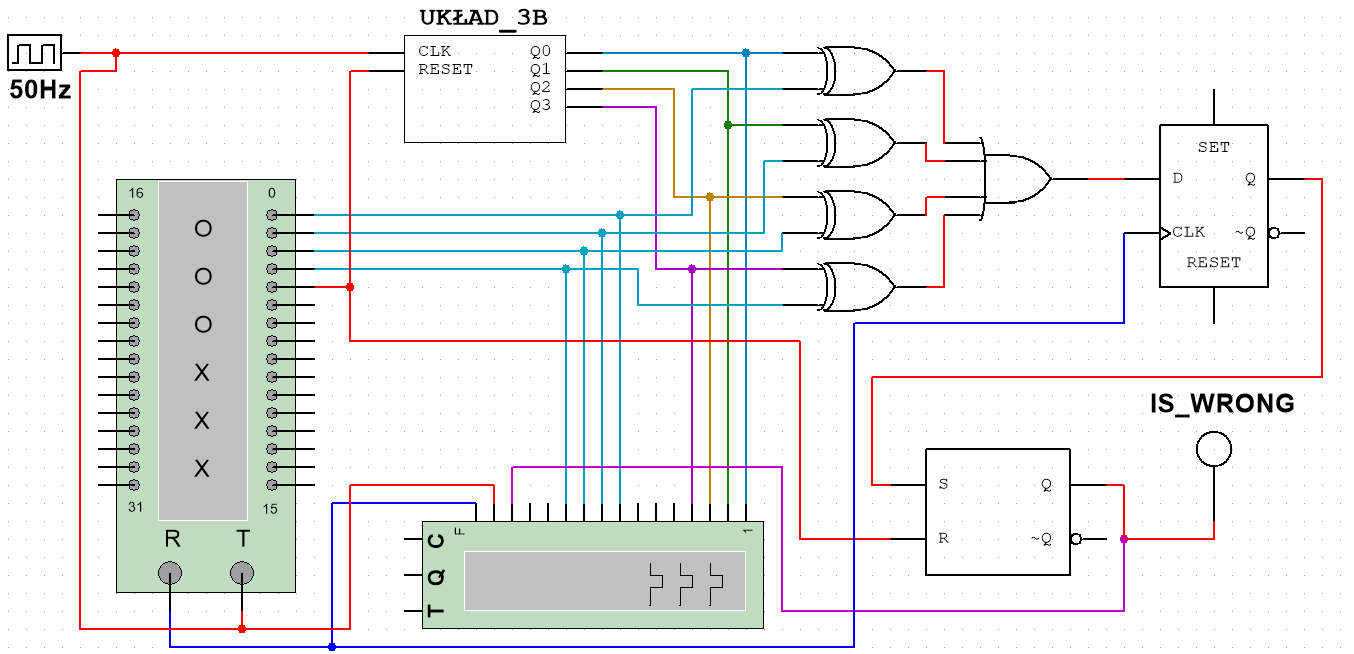
\includegraphics[width=\textwidth]{3b_test.png}
    \caption{Układ testujący}
\end{figure}

\begin{figure}[H]
    \centering
    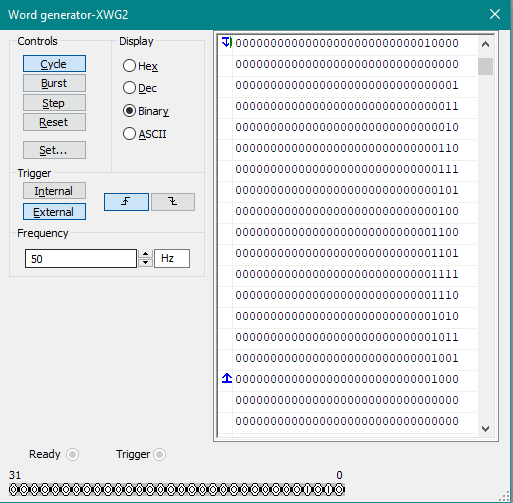
\includegraphics[width=0.7\textwidth]{3b_test_gen.png}
    \caption{Generator słów}
\end{figure}

\begin{figure}[H]
    \centering
    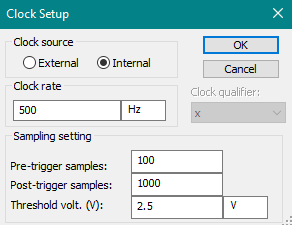
\includegraphics[width=0.6\textwidth]{3b_impl_ana_opc.png}
    \caption{Opcje analizatora}
\end{figure}

\begin{figure}[H]
    \centering
    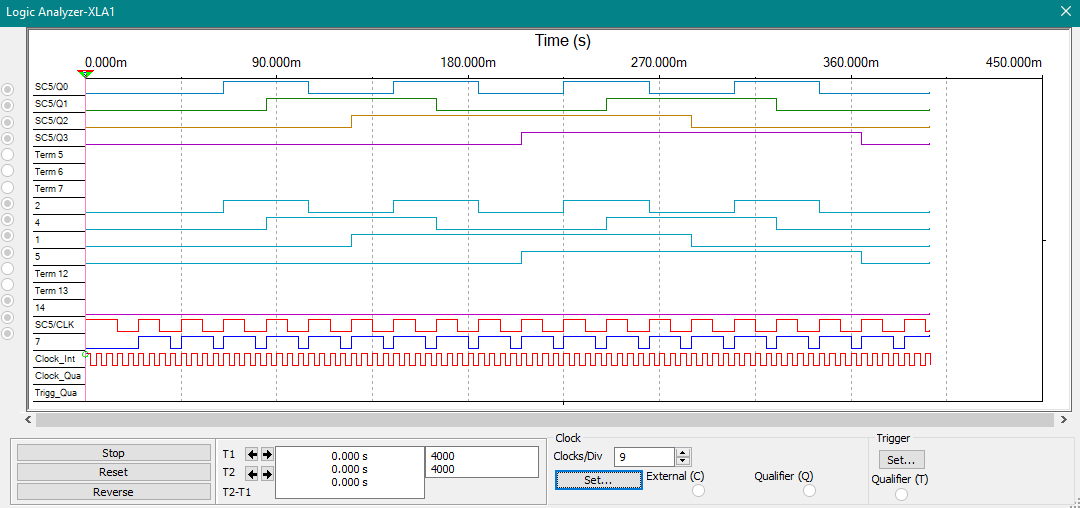
\includegraphics[width=\textwidth]{3b_test_ana.png}
    \caption{Analizator stanów logicznych}
\end{figure}

\subsection{Wnioski}
\begin{itemize}
    \item
    Alternatywnym podejściem mogłoby być wykorzystanie innego typu przerzutników np. przerzutników JK (wówczas trzeba by jednak
    liczyć osiem zamiast czterech funkcji, bo bramka JK ma 2 wejścia) lub przerzutników typu T, które wydają się bardziej adekwatne.
    Podejście z przerzutnikiem T wymagałoby skonstruowania funkcji $T_0$, $T_1$, $T_2$, $T_3$, np. tabela Karnough dla $T_0$:

    \begin{figure}[H]
        \centering
        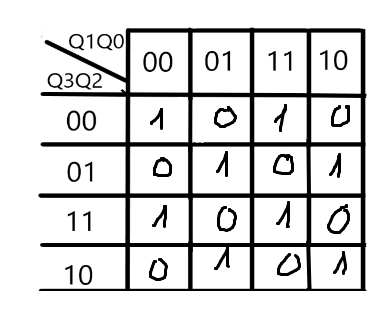
\includegraphics[width=0.6\textwidth]{3b_alt.jpg}
        \caption{Tabela Karnough dla $T_0$}
    \end{figure}

    $$T_0 = \overline{Q_3}\:\overline{Q_2}\:\overline{Q_1}\:\overline{Q_3} + \overline{Q_3}\:\overline{Q_2}Q_1Q_0 + ... + 
    Q_3\overline{Q_2}Q_1\overline{Q_0}$$

    Jak widać, nie można zaznaczyć żadnej grupy większej niż jedna wartość, więc funkcja $T_0$ składałaby się z sumy ośmiu elementów,
    co wymaga większej liczby bramek i jest bardziej podatne na błędy w implementacji.

    \item
    Licznik synchroniczny w kodzie Graya, podobnie jak zwyczajny licznik binarny, może służyć jako dzielnik częstosliwości,
    jednak w tym przypadku częstotliwość sygnału na wyjściu najmniej znaczącego bitu będzie czterokrotnie mniejsza niż na wejściu,
    na wyjściu drugiego bitu ośmiokrotnie mniejsza itd.
    \item
    Przypuśćmy, że układ korzystający z licznika Graya służy do sterowania prądem przepływającym przez np. diodę LED. Użytkownik
    może naciskać przycisk tak żeby zwiększyć jasność diody (natężenie na diodzie = wyjście z licznika $\cdot$ pewne natężenie bazowe).
    Po tym gdy użytkownik znajdzie się w najwyższej pozycji licznika (np. 10) licznika wraca do pozycji minimalnej.

    \begin{figure}[H]
        \centering
        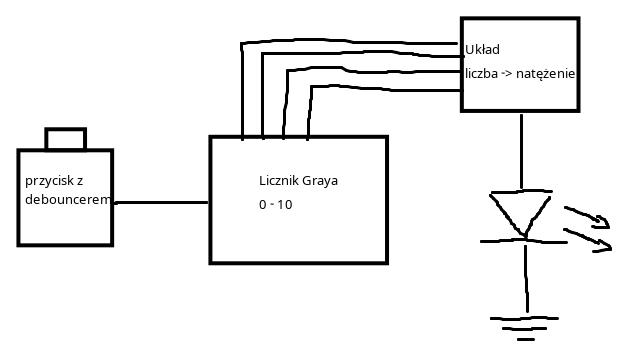
\includegraphics[width=0.6\textwidth]{3b_przyklad.jpg}
        \caption{Przykład - układ sterujący jasnością diody}
    \end{figure}

    Gdyby używać licznika binarnego, wówczas istnieje ryzyko, że podczas zmiany stanów dioda chwilowo znajdzie się w stanie zabronionym
    (np. 0111 $\rightarrow$ 1000 znajdzie się w stanie 1111), na diodę podane zostanie natężenie większe niż może przyjąć i dioda się przepali.
    Przy użyciu licznika w kodzie Graya podobne zagrożenie nie istnieje.

\end{itemize}

\pagebreak
\section{Ćwiczenie \textit{3c}}
Ideą ćwiczenia jest, bazując na przerzutnikach "D", zaprojektowanie, zbudowanie i przetestowanie automatu realizującego detekcję litery Q
przekazywanej alfabetem Morsa, czyli sekwencji bitów: "— — • —". Za kreskę nalezy przyjąć stan logiczny '1', a za kropkę stan logiczny
'0'. Należy również zaproponować własny, ale skuteczny i praktyczny sposób wprowadzania do urządzenia sygnału wejściowego.

\begin{figure}[H]
    \centering
    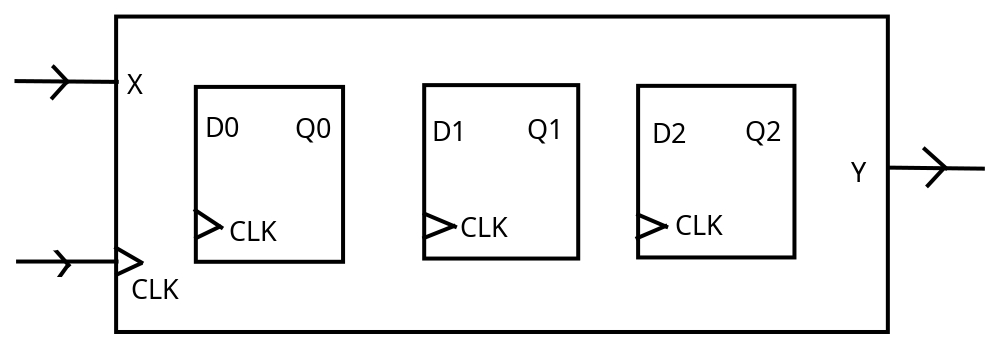
\includegraphics[width=0.6\textwidth]{3c_idea.jpg}
    \caption{Układ 3c}
\end{figure}

\subsection{Rozwiązanie teoretyczne}
Sekwencja, którą trzeba wykryć, to "1101", na tej podstawie zaprojektować można automat wykrywający owe słowo:

\begin{figure}[H]
    \centering
    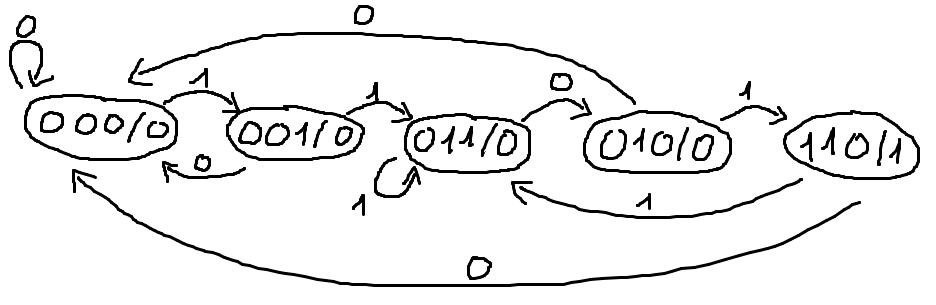
\includegraphics[width=\textwidth]{3c_automaton.jpg}
    \caption{Automat wykrywający słowo "1101"}
\end{figure}

Na podstawie automatu można stworzyć tabelę kolejnych stanów oraz tabelę dla Y:

\begin{figure}[H]
    \centering
    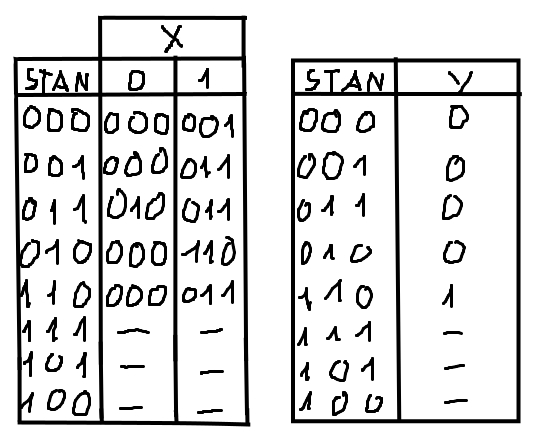
\includegraphics[width=0.7\textwidth]{3c_tabela.jpg}
    \caption{Tabela kolejnych stanów automatu oraz tabela Y}
\end{figure}

Pozostaje skonstruować tabele Karnough (STAN = $Q_2Q_1Q_0$):

\begin{figure}[H]
    \centering
    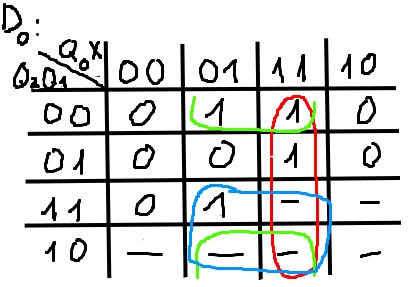
\includegraphics[width=0.6\textwidth]{3c_karn_0.jpg}
    \caption{Tabela Karnough dla $D_0$}
\end{figure}

$$D_0 = \Cline[red]{Q_0X} +
\Cline[green]{X\overline{Q_1}} + 
\Cline[blue]{XQ_2}$$

\begin{figure}[H]
    \centering
    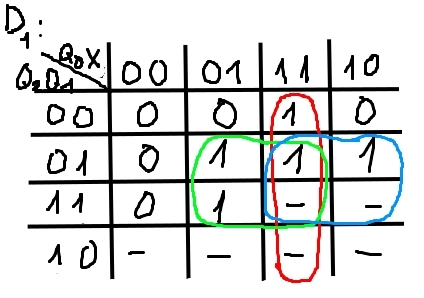
\includegraphics[width=0.6\textwidth]{3c_karn_1.jpg}
    \caption{Tabela Karnough dla $D_1$}
\end{figure}

$$D_1 = \Cline[red]{Q_0X} +
\Cline[green]{XQ_1} + 
\Cline[blue]{Q_0Q_1}$$

\begin{figure}[H]
    \centering
    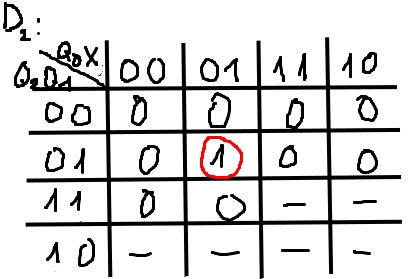
\includegraphics[width=0.6\textwidth]{3c_karn_2.jpg}
    \caption{Tabela Karnough dla $D_2$}
\end{figure}

$$D_2 = \Cline[red]{\overline{Q_0}X\overline{Q_2}Q_1}$$

Oraz tabela Karnough dla Y:

\begin{figure}[H]
    \centering
    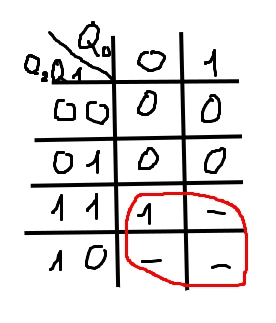
\includegraphics[width=0.4\textwidth]{3c_karn_y.jpg}
    \caption{Tabela Karnough dla $Y$}
\end{figure}

$$Y = \Cline[red]{Q_2}$$

\subsection{Implementacja w programie Multisim}

\begin{figure}[H]
    \centering
    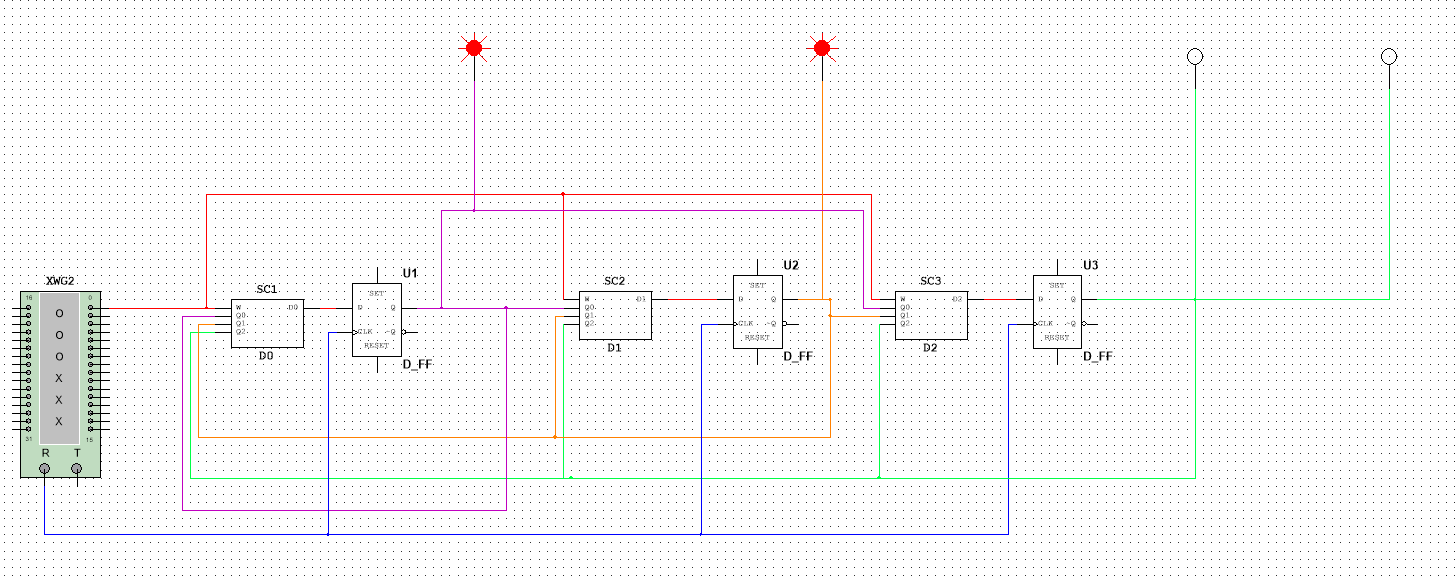
\includegraphics[width=\textwidth]{3c_impl.png}
    \caption{Implementacja w programie Multisim}
\end{figure}

$$D_0 = Q_0X +
X\overline{Q_1} + 
XQ_2$$

\begin{figure}[H]
    \centering
    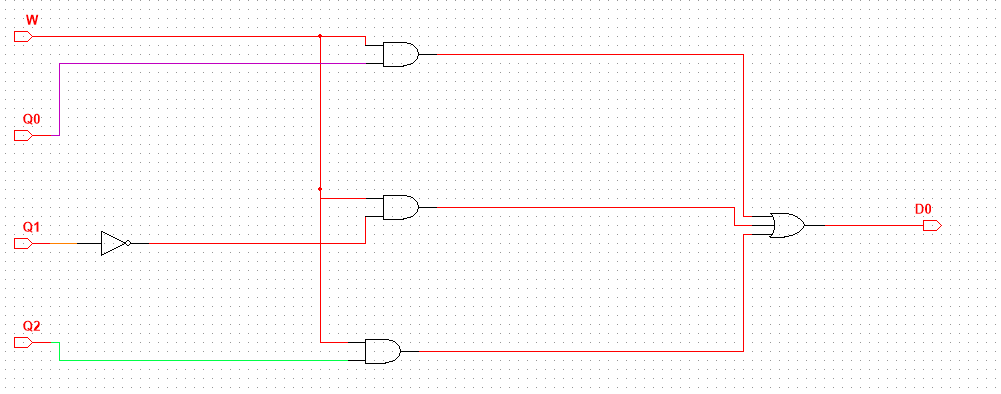
\includegraphics[width=\textwidth]{3c_impl_0.png}
    \caption{Podukład $D_0$}
\end{figure}

\pagebreak
$$D_1 = Q_0X +
XQ_1 + 
Q_0Q_1$$

\begin{figure}[H]
    \centering
    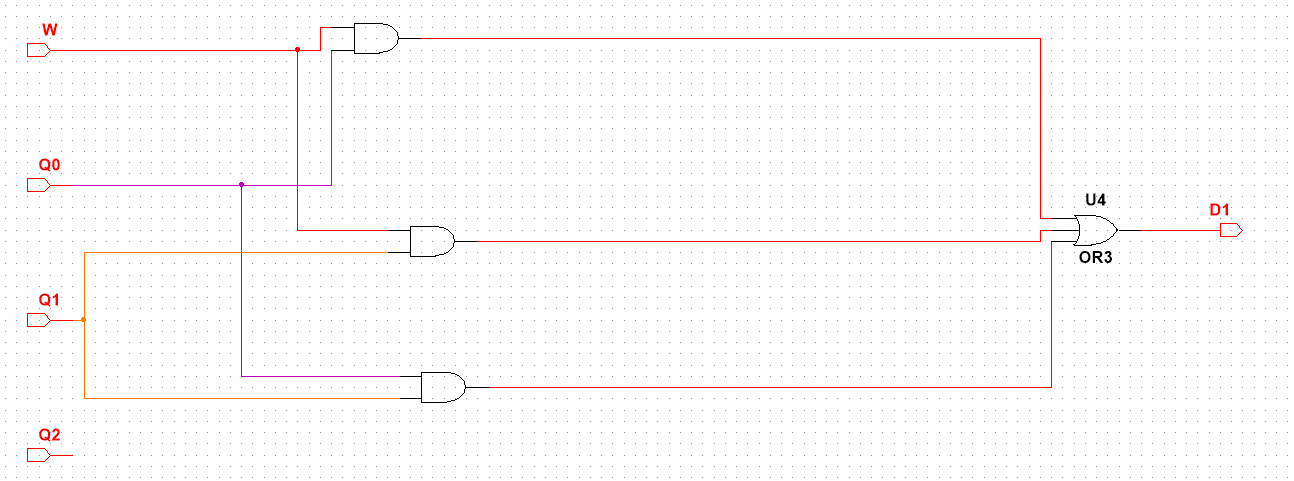
\includegraphics[width=\textwidth]{3c_impl_1.png}
    \caption{Podukład $D_1$}
\end{figure}

$$D_2 = \overline{Q_0}X\overline{Q_2}Q_1$$

\begin{figure}[H]
    \centering
    \includegraphics[width=\textwidth]{3c_impl_2.png}
    \caption{Podukład $D_2$}
\end{figure}

\pagebreak
Poniżej układ testujący:

\begin{figure}[H]
    \centering
    \includegraphics[width=\textwidth]{3c_test.png}
    \caption{Układ testujący}
\end{figure}

\begin{figure}[H]
    \centering
    \includegraphics[width=\textwidth]{3c_test_ana.png}
    \caption{Analizator stanów logicznych w układzie testującym}
\end{figure}

\begin{figure}[H]
    \centering
    \includegraphics[width=0.8\textwidth]{3c_test_gen.png}
    \caption{Generator słów w układzie testująym}
\end{figure}

\begin{figure}[H]
    \centering
    \includegraphics[width=0.6\textwidth]{3c_test_ana_ust.png}
    \caption{Ustawienia analizatora stanów logicznych}
\end{figure}

\subsection{Wnioski}
\begin{itemize}
    \item
    Prostym, a praktycznym sposobem podawania sygnału wejściowego byłoby zastosowanie przełącznika i przycisku:
    przełącznik określałby stan kolejnego symbolu (włączony - 1, wyłączony - 0), a drugi pełniłby rolę manualnego zegara.

    \begin{figure}[H]
        \centering
        \includegraphics[width=0.6\textwidth]{3c_wpr.jpg}
        \caption{Wprowadzanie sygnału}
    \end{figure}

    \item
    W naszym podejściu kolejne stany oznaczone kolejnymi liczbami w kodzie Graya (przypadłość po ćwiczeniu 3b). Alternatywnie, można
    opisać by je kolejnymi liczbami zapisanymi binarnie (000, 001, 010, 011, 100). Wówczas tabele Karnough, a co za tym idzie,
    wzory byłyby inne niż obecnie.

    \begin{figure}[H]
        \centering
        \includegraphics[width=0.6\textwidth]{3c_alt.jpg}
        \caption{Alternatywne oznaczenia stanów automatu}
    \end{figure}

    \begin{figure}[H]
        \centering
        \includegraphics[width=0.6\textwidth]{3c_alt_1.jpg}
        \caption{Alternatywna tabela Karnough $D_0$}
    \end{figure}

    $$D_0 = \overline{Q_0}X\overline{Q_2}$$

    \item
    Hipotetycznym scenariuszem, w którym układ byłby przydatny, to wykrywanie sygnału wysyłanego przez pewną maszynę. Przypuśćmy, że
    maszyna może wysyłać różne sygnały, np. o tym, że kończy się materiał, z którego korzysta. Jednym z sygnałów wysyłanych może być sygnał
    stop (1101), wysyłany w przypadku, gdy np. maszyna się przegrzewa. Układ wykrywa ten sygnał i odłącza maszynę od prądu.

    \begin{figure}[H]
        \centering
        \includegraphics[width=0.7\textwidth]{3c_przyklad.jpg}
        \caption{Maszyna wysyłająca sygnały}
    \end{figure}

\end{itemize}

\end{document}